\documentclass{article}
\usepackage{amsmath}
\usepackage{tikz}
\begin{document}

\title{Electricity and Magnetism - Lecture 6 Notes}
\author{Joshua Clement}
\maketitle


\section*{Electric Field Calculations for Different Geometries}
\begin{itemize}
    \item \textbf{Points, Lines, and Planes}:
    \begin{itemize}
        \item \textbf{Point Charge}: Electric field radiates outward from the point

        (\(E = \frac{1}{r^2})\).
        \item \textbf{Infinite Line Charge}: Electric field extends radially outward, decreases with distance (\(E = \frac{1}{r})\).
        \item \textbf{Infinite Plane Charge}: Electric field is constant at all points above or below the plane (\(E = Constant\)).
    \end{itemize}
\end{itemize}

\section*{Electric Field Along the Axis of a Ring}

\begin{figure}[h!]
    \centering
    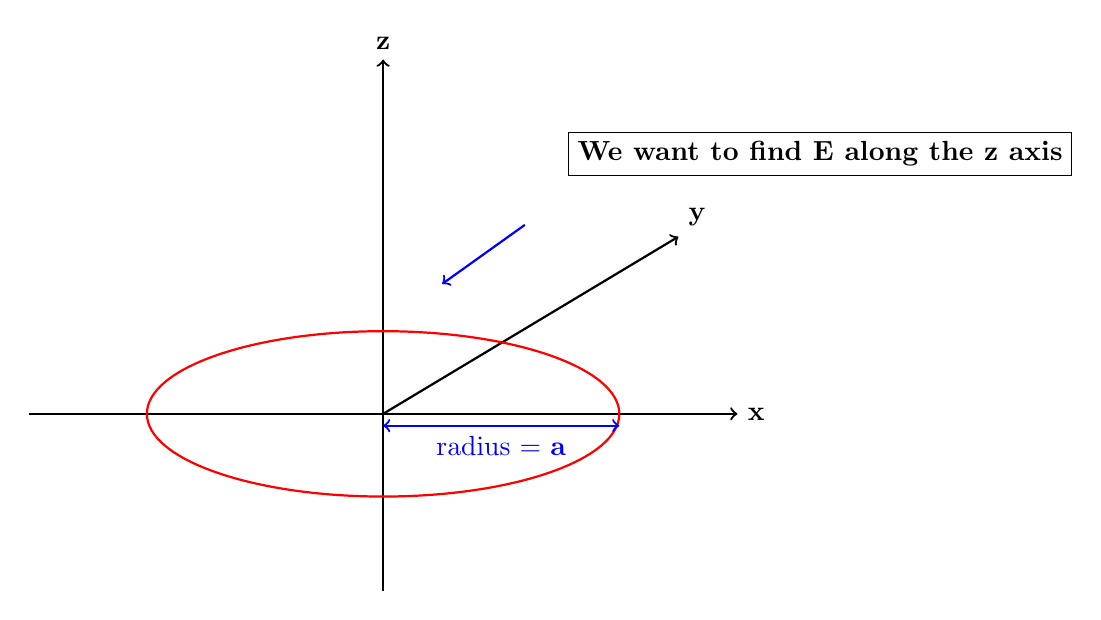
\begin{tikzpicture}[scale=1.5]
        % Draw the coordinate axes
        \draw[->, thick] (-3, 0) -- (3, 0) node[right] {\textbf{x}};
        \draw[->, thick] (0, -1.5) -- (0, 3) node[above] {\textbf{z}};
        \draw[->, thick] (0, 0) -- (2.5, 1.5) node[above right] {\textbf{y}};

        % Draw the ring in the xy-plane
        \draw[red, thick] (0, 0) ellipse (2 and 0.7);

        % Draw the radius annotation
        \draw[<->, blue, thick] (0, -0.1) -- (2, -0.1) node[midway, below] {radius = \textbf{a}};

        % Draw the annotation box and arrow
        \draw[->, thick, blue] (1.2, 1.6) -- (0.5, 1.1);
        \node[draw] at (3.7, 2.2) {
            \textbf{We want to find} \\
            \textbf{ E along the z axis}
        };

    \end{tikzpicture}
    \caption{Illustration of finding the electric field along the z-axis of a charged ring.}
    \label{fig:ring_field}
\end{figure}

\begin{itemize}
    \item Goal: Find the electric field (\(E\)) along the \textbf{z-axis} of a ring with total charge \(Q\) and radius \(a\).
    \item \textbf{Symmetry Considerations}:
    \begin{itemize}
        \item Only the \textbf{z-component} of the electric field survives due to symmetry.
    \end{itemize}
    \item \textbf{Electric Field Contribution} (\(\Delta E_z\)) from a small charge element (\(\Delta q\)) on the ring:
    \[
    \Delta E_z = \frac{1}{4 \pi \epsilon_0} \frac{z \Delta q}{(a^2 + z^2)^{\frac{3}{2}}}
    \]
    \item \textbf{Total Electric Field}:
    \[
    E_{\text{tot}} = \int_{\text{ring}} \Delta E_z = \frac{1}{4 \pi \epsilon_0} \frac{Q z}{(a^2 + z^2)^{\frac{3}{2}}} \hat{z}
    \]
\end{itemize}

\section*{Electric Field Along the Axis of a Disk}
\begin{itemize}
    \item Goal: Find the electric field (\(E\)) along the \textbf{z-axis} of a disk with total charge \(Q\) and radius \(R\).
    \item \textbf{Symmetry Considerations}:
    \begin{itemize}
        \item Only the \textbf{z-component} of the electric field survives due to symmetry.
    \end{itemize}
    \item \textbf{Surface Charge Density} (\(\sigma\)):
    \[
    \sigma = \frac{Q}{\pi R^2}
    \]
    \item \textbf{Electric Field Contribution} (\(\Delta E_z\)):
    \[
        \Delta E_z = \frac{1}{4 \pi \epsilon_0} \frac{z \Delta q}{(a^2 + z^2)^{\frac{3}{2}}}
    \]
    \item \textbf{Total Electric Field}:
    \[
    E_{\text{tot}} = \frac{1}{2 \epsilon_0} \left(\frac{Q}{\pi R^2}  \right) \left[ 1 - \frac{z}{\sqrt{R^2 + z^2}} \right] \hat{z}
    \]
\end{itemize}

\section*{Field of an Infinite Plane}
\begin{itemize}
    \item \textbf{Infinite Plane with Uniform Charge Density} (\(\sigma\)):
    \item The electric field is \textbf{constant} at all points on either side of the plane:
    \[
    E = \frac{\sigma}{2 \epsilon_0}
    \]
    \item This field is independent of the distance from the plane.
\end{itemize}

\section*{Field of Two Infinite Planes}

\begin{figure}[h!]
    \centering
    \begin{tikzpicture}[scale=1.5]
        % Define styles for the arrows
        \tikzset{
            black arrow/.style={->, thick, black}
        }

        % Draw the two parallel plates
        \draw[thick, red] (2, -3) -- (2, 3);
        \draw[thick, blue] (4, -3) -- (4, 3);

        % Draw electric field arrows between the plates
        \foreach \y in {-2.5, -2, -1.5, -1, -0.5, 0, 0.5, 1, 1.5, 2, 2.5} {
            \draw[black arrow] (2.2, \y) -- (3.8, \y);
        }

        % Labels for the electric fields
        \node at (5, 0) {$E = 0$};
        \node at (1, 0) {$E = 0$};
        \node at (3, 3.5) {$E = \frac{\sigma}{\epsilon_0}$};

    \end{tikzpicture}
    \caption{Electric field between two infinite parallel plates. Fields inside add up, while fields outside cancel.}
    \label{fig:parallel_plates_field}
\end{figure}

\begin{itemize}
    \item \textbf{Two Infinite Planes with Opposite Charge Density}:
    \item \textbf{Superposition Principle}:
    \begin{itemize}
        \item The field between the planes \textbf{adds}, resulting in a net field of:
        \[
        E_{\text{net}} = \frac{\sigma}{\epsilon_0}
        \]
        \item Outside the planes, the fields \textbf{cancel} each other.
    \end{itemize}
\end{itemize}

\section*{Key Concepts}
\begin{itemize}
    \item \textbf{Symmetry} plays a crucial role in simplifying electric field calculations.
    \item For \textbf{rings and disks}, only the component along the axis survives.
    \item For \textbf{infinite planes}, the electric field is constant regardless of distance from the plane.
    \item \textbf{Superposition} helps determine the net field when dealing with multiple charge distributions.
\end{itemize}


\end{document}